% This file was converted to LaTeX by Writer2LaTeX ver. 1.2
% see http://writer2latex.sourceforge.net for more info
\documentclass[a4paper]{article}
\usepackage[ascii]{inputenc}
\usepackage[T1]{fontenc}
\usepackage[romanian,english,ngerman]{babel}
\usepackage{amsmath}
\usepackage{amssymb,amsfonts,textcomp}
\usepackage{color}
\usepackage{array}
\usepackage{hhline}
\usepackage{hyperref}
\hypersetup{pdftex, colorlinks=true, linkcolor=blue, citecolor=blue, filecolor=blue, urlcolor=blue, pdftitle=, pdfauthor=, pdfsubject=, pdfkeywords=}
\usepackage[pdftex]{graphicx}
% List styles
\newcommand\liststyleLv{%
\renewcommand\theenumi{\arabic{enumi}}
\renewcommand\theenumii{\arabic{enumii}}
\renewcommand\theenumiii{\arabic{enumiii}}
\renewcommand\theenumiv{\arabic{enumiv}}
\renewcommand\labelenumi{\theenumi.}
\renewcommand\labelenumii{\theenumii.}
\renewcommand\labelenumiii{\theenumiii.}
\renewcommand\labelenumiv{\theenumiv.}
}
\newcommand\liststyleLSi{%
\renewcommand\theenumi{\arabic{enumi}}
\renewcommand\theenumii{\arabic{enumii}}
\renewcommand\theenumiii{\arabic{enumiii}}
\renewcommand\theenumiv{\arabic{enumiv}}
\renewcommand\labelenumi{\theenumi.}
\renewcommand\labelenumii{\theenumii.}
\renewcommand\labelenumiii{\theenumiii.}
\renewcommand\labelenumiv{\theenumiv.}
}
% Page layout (geometry)
\setlength\voffset{-1in}
\setlength\hoffset{-1in}
\setlength\topmargin{0.7874in}
\setlength\oddsidemargin{0.7874in}
\setlength\textheight{10.1177in}
\setlength\textwidth{6.692499in}
\setlength\footskip{0.0cm}
\setlength\headheight{0cm}
\setlength\headsep{0cm}
% Footnote rule
\setlength{\skip\footins}{0.0469in}
\renewcommand\footnoterule{\vspace*{-0.0071in}\setlength\leftskip{0pt}\setlength\rightskip{0pt plus 1fil}\noindent\textcolor{black}{\rule{0.25\columnwidth}{0.0071in}}\vspace*{0.0398in}}
% Pages styles
\makeatletter
\newcommand\ps@Standard{
  \renewcommand\@oddhead{}
  \renewcommand\@evenhead{}
  \renewcommand\@oddfoot{}
  \renewcommand\@evenfoot{}
  \renewcommand\thepage{\arabic{page}}
}
\makeatother
\pagestyle{Standard}
\title{}
\author{}
\date{2013-04-08}

%Cosmin
\setlength{\tabcolsep}{50pt}

\begin{document}
{\raggedleft\bfseries
MACHETA 3
\par}

{\bfseries
Contractor: \foreignlanguage{romanian}{Universitatea din Bucure\c{s}ti}}

{\textbf{Cod fiscal: 45055002}


\bigskip


\bigskip


\bigskip


\bigskip

{\bfseries

\begin{tabular}{@{}l l}
Avizat,&De acord,\\
Comisia de monitorizare&DIRECTOR PLAN SECTORIAL\\
\end{tabular}
}

\bigskip

PRE\c{S}EDINTE

Prof.univ.dr. Tudor Prisecaru

\bigskip

MEMBRII

\bigskip

\bigskip

MONITOR PROIECT

Daniela Dinic\u{a}

\bigskip

\bigskip

\bigskip

\bigskip

{\centering\bfseries
RAPORT DE ACTIVITATE AL FAZEI
\par}


\bigskip


\bigskip

{\bfseries
Contractul nr.: 5S / 27.07.2012}

{
\textbf{Proiectul: }
\textit{`` Sistem informatic integrat pentru identificarea, arhivarea \c{s}i diseminarea bazelor de date \c{s}i a indicatorilor din
cercet\u{a}rile sociale ''}}

\bigskip

%TODO Titlul fazei !
{
\textbf{Faza: }
Nr. II cu titlul
\textit{`` Sistemul de acces la date ''}}

{\textbf{Termen:} 10.04.2013}

\bigskip
{\bfseries 
1. Obiectivul proiectului}

{
\foreignlanguage{english}{Realizarea }\foreignlanguage{romanian}{unei arhive electronice integrate care s\u{a}
con\c{t}in\u{a} \c{s}i s\u{a} distribuie c\^at mai multe dintre datele sociologice acumulate \^in Rom\^ania.}}

{\selectlanguage{romanian}
Sistemul trebuie s\u{a} ofere cercet\u{a}torilor \^in domeniul \c{s}tiin\c{t}elor sociale instrumentele necesare pentru
trecerea \^in revist\u{a}, compararea, sintetizarea, ad\u{a}ugarea datelor sociologice de interes. Operatorii interni
ai arhivei vor c\u{a}uta, identifica \c{s}i acumula date sociologice disponibile \^in Rom\^ania.}

{\selectlanguage{romanian}
Arhiva va fi integrat\u{a} \^in Consiliul European al Arhivelor de Date Sociale (CESSDA) asigur\^andu-se un schimb
continuu bidirec\c{t}ional de informa\c{t}ie.}

\bigskip
{\bfseries
2. Rezultate preconizate pentru atingerea obiectivului}

\liststyleLv
\begin{enumerate}
\item {
Sistem informatic de arhivare (stocare, catalogare plus proceduri \c{s}i capacit\u{a}\c{t}i de identificare \c{s}i
accesare) \foreignlanguage{romanian}{\c{s}}i diseminare a datelor sociale produse de pia\c{t}a cercet\u{a}rii sociale
din Rom\^ania.}
\item {
Asigurarea procedurilor de securizare a accesului la datele arhivate, ca urmare a investi\c{t}iilor \^in hardware
\foreignlanguage{romanian}{\c{s}}i software pe parcursul proiectului;}
\item {
\foreignlanguage{romanian}{Arhiva }va func\c{t}iona inclusiv ca o banc\u{a} de date sociale, dat fiind faptul c\u{a}
produc\u{a}torii de date nu au nici capacit\u{a}\c{t}ile tehnice nici \foreignlanguage{romanian}{cunoa\c{s}terea}
necesar\u{a} depozit\u{a}rii, catalog\u{a}rii \c{s}i acces\u{a}rii cercet\u{a}rilor realizate, pe termen lung;}
\item {
Facilitarea accesului comunit\u{a}\c{t}ii de cercetare din Rom\^ania la datele produse \^in ultimii 20 de ani pe
pia\c{t}a na\c{t}ional\u{a} de profil, dar \c{s}i la cele europene, ca urmare a conect\u{a}rii arhivei la CESSDA-ERIC
(arhiva fiind deja membru al CESSDA);}
\item {
Facilitarea accesului comunit\u{a}\c{t}ii de cercetare interna\c{t}ionale la datele produse \^in Rom\^ania prin
intermediul CESSDA va aduce de asemenea mari beneficii interna\c{t}ionaliz\u{a}rii cercet\u{a}rii sociale din
Rom\^ania;}
\item {
Articole de specialitate/comunic\u{a}ri \c{s}tiin\c{t}ifice menite a face cunoscute pe plan na\c{t}ional \c{s}i
interna\c{t}ional beneficiile sistemului implementat ca urmare a derul\u{a}rii sale.}
\end{enumerate}

\bigskip
{\bfseries
3. Obiectivul fazei}

{\selectlanguage{romanian}
%TODO Obiectivul fazei, cf. documentatiei proiectului 
Implementarea sistemului de acces la date}

\bigskip
{\bfseries
4. Rezultate preconizate pentru atingerea obiectivului fazei}

{\selectlanguage{romanian}
%TODO Rezultate - cf. documentatiei proiectului
Implementarea setului de biblioteci software care permit accesul (scrierea, citirea si modificarea) datelor care compun
arhiva RODA. }

\bigskip
{\bfseries
5. Rezumatul fazei}

{\selectlanguage{english}\bfseries\color[rgb]{0.0,0.0,0.039215688}
Sistemul de acces la date}

{
Sistemul de acces la date este ansamblul software RODA care asigura accesul tuturor celorlalte componente ale arhivei
electronice la datele propriu-zise. Acesta este pozitionat intre orice componenta care solicita citirea sau scrierea
datelor si oricare dintre elementele de stocare ale RODA (baza de date, index, fisiere statice).}

\bigskip

{
Sistemul de acces la date trebuie sa se constituie intr-un model unitar care strange laolalta toate metodele de
comunicare si modificarile automate facute asupra datelor la intrarea sau iesirea din baza de date, index sau fisiere
statice.}

{\selectlanguage{english}\bfseries\color[rgb]{0.0,0.0,0.039215688}
Structura si componente}

{
\textbf{Pachetul RODA} reprezinta principala componenta a sistemului de acces la date. Toate celelalte componente sunt
apelabile prin intermediul metodelor RODA, acesta reprezentand ``poarta de intrare'' in sistem.}

\bigskip

{
\textbf{RODA::Config} reprezinta pachetul care se ocupa de citirea si interpretarea fisierului de configurare a
aplicatiei, in care sunt scrise informatiile esentiale, de care sistemul are nevoie pentru initializare inainte de a
putea accesa serverul de baze de date. RODA::Config este disponibil (importat) atat la nivelul pachetului principal
(RODA) cat si la nivelul pachetului RODADB care reprezinta maparea basei de date SQL.}


\bigskip

{
\textbf{RODA::Log} reprezinta pachetul care se ocupa de acumularea si distributia mesajelor jurnalului aplicatiei.
Acestea pot fi trimise concomitent catre mai multe sisteme de acumulare (sistem de fisiere, baza de date, etc.). Ca si
RODA::Config el este disponibil atat la nivelul modulului principal cat si la nivelul maparii schemei bazei de date
RODADB.}

\bigskip

{\centering  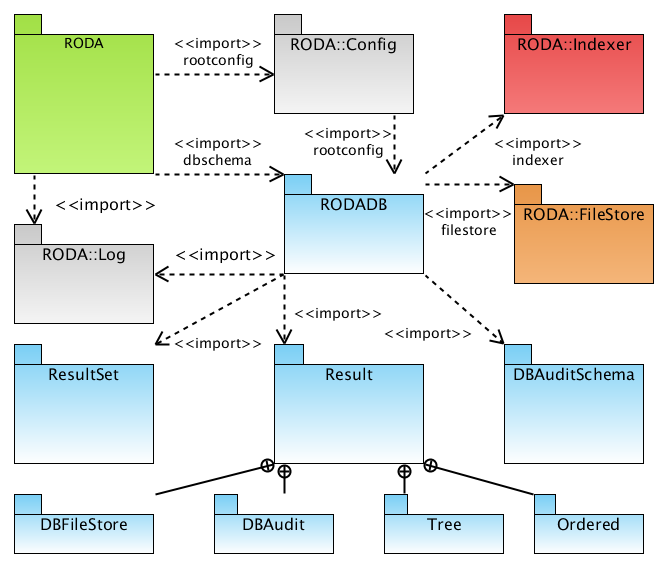
\includegraphics[width=6.9272in,height=5.9583in]{rodaraportfaza2-img001.png} \par}
{
\textbf{RODA::RODADB} este componenta principala al sistemului de acces la date. Acesta se bazeaza pe o mapare
relational-obiectuala extinsa cu componente necesare. RODA::RODADB contine elementele principale necesare accesului la
datele relationale, metode care permit introducerea datelor in tabele, citirea lor, modificarea celor existente,
stergere, etc. Clasele au fost extinse prin adaugarea de metode specifice care permit introducerea / stergerea
structurilor de informatii care traverseaza mai multe tabele (ex: introducerea unei persoane sau introducerea unei
organizatii).}


\bigskip

{
\textbf{RODA::Indexer} este componenta care se ocupa de relatia dintre baza de date relationala si indexul de cautare
(Apache Solr). Contine metode care sincronizeaza datele din baza de date cu cele din index si care introduc date in
index.}


\bigskip

{
\textbf{RODADB::Result} reprezinta o clasa de baza care are cate o clasa subordonata pentru fiecare tabel din baza de
date SQL. Aceste clase contin metodele pentru accesarea unui singur rand din tabelul corespunzator.}


\bigskip

{
\textbf{RODADB::ResultSet} reprezinta o clasa de baza in care se gasesc metode pentru accesarea colectiilor de randuri
(e.g.: Search).}


\bigskip

{
\textbf{RODA::Filestore} reprezinta un modul care permite accesarea fisierelor statice. FileStore defineste un volum
care reprezinta un anumit spatiu pe sistemul de fisiere. In acest volum, cu ajutorul functionalitatilo FileStore, se
pot pune si sterge fisiere, se pot afla, printr-un sistem de plugin-uri, caracteristicile fisierelor cunoscute
(imagini, pdo umenteetc.). RODADB poate utiliza un numar nelimitat de FileStore-uri d,ar trebuie sa aiba cel putin
unul.}


\bigskip

{
\textbf{DBAuditSchema} reprezinta o colectie de functii de baza pentru sistemul de audit al bazei de date. Acestea
adauga metodele necesare pentru audit la functiile de baza ale sistemului de mapare relational-obiectuala (inceput de
tranzactie, finalizare a tranzactiei, rollback).}


\bigskip

{
\textbf{DBAudit} reprezinta componenta care, lucrand impreuna cu DBAuditSchema, capteaza solicitarile de introducere,
modificare si stergere a datelor din tabelele monitorizate si adauga intr-un set de tabele speciale informatiile de
audit. Pe baza acestora se poate urmari istoricul tuturor modificarilor facute asupra bazei de date si, in cazul unor
modificari nedorite, se pot restaura datele.}


\bigskip

{
\textbf{DBFileStore} reprezinta o componenta care permite transferul automat al fisierelor referite in coloanele
\ tabelelor bazei de date. In legatura directa cu RODA::FileStore, DBFileStore permite transferul transparent al
fisierelor introduse in coloanele tabelelor intr-o cale standard definita in volum. In baza de date se va stoca numele
fisierului iar, la citirea acestuia, DBFileStore va transforma automat inregistrarea atasand metodele necesare pentru a
obtine detalii despre fisierul respectiv.}


\bigskip

{
Alte componente ce trebuie evidentiate sunt:}

{
\textbf{{}- Tree} reauga o serie de metode care permit lucrul direct cu tabele auto-referentiate.}

{
{}- \textbf{Ordered} adauga o serie de metode care permit lucrul cu tabele care contin informatii secventiale (o coloana
speciala de ordonare). Ordered permite atat ordonarea totala (pe tot tabelul) cat si ordonarea grupata (in functie de
alta coloana din tabel).}


\bigskip

{
Pentru a permite interoperabilitatea aplicatiei RODA cu institutii similare din alte tari membre U.E. (e.g. GESIS, NSD,
DDA), cu alte aplicatii software (e.g. MISSY, DdiEditor, Nesstar) si proiecte europene (e.g. {\textquotedbl}Data
without Boundaries{\textquotedbl}), precum si functionalitati relative la CESSDA (e.g. autentificare cu Shibboleth) si
DDI-Alliance (XML repository, RDF export), includem in documentatie un set de componente dezvoltate in Java si Spring
framework, complementare unui sistem echivalent de acces la date.}


\bigskip

{
Detaliile de implementare a componentelor de mai sus sunt prezentate pe larg in Anexa 1.}

\bigskip

{\selectlanguage{english}\bfseries\color[rgb]{0.0,0.0,0.039215688}
Securitatea aplica\c{t}iei RODA}

{
Securitatea datelor stocate in arhiva RODA este deosebit de important\u{a}. O parte dintre datele stocate vor fi cu
acces limitat, o parte cu acces aproape interzis (acces exclusiv). \^Intreaga infrastructur\u{a} hardware \c{s}i
software trebuie s\u{a} fie proiectat\u{a} astfel \^inc\^at s\u{a} asigure protec\c{t}ia total\u{a} a datelor.}

{\selectlanguage{english}\bfseries\itshape\color[rgb]{0.0,0.0,0.039215688}
Men\c{t}inerea integrit\u{a}\c{t}ii datelor}

{
Men\c{t}inerea integrit\u{a}\c{t}ii datelor se refer\u{a} la ansamblul de m\u{a}suri luate pentru a evita pierderea
lor, par\c{t}ial\u{a} sau total\u{a}, indiferent de modul \^in care aceasta poate sa apar\u{a}.}


\bigskip

{
Riscurile de pierdere a datelor provin de obicei din urm\u{a}toarele accidente:}


\bigskip

\liststyleLSi
\begin{enumerate}
\item {
Disfunc\c{t}ionalit\u{a}\c{t}i ale infrastructurii hardware (hard-diskuri defecte, sisteme de date corupte de erori
software, manevrarea excesiva de c\u{a}tre utilizatori cu drepturi ridicate a func\c{t}iilor de cur\u{a}\c{t}are).
Principala protec\c{t}ie \^impotriva acestui grup de probleme o reprezint\u{a} redundan\c{t}a datelor \c{s}i
backup-ul.}
\item {
Alte situa\c{t}ii de for\c{t}\u{a} major\u{a} (distrugeri ale serverelor determinate de calamit\u{a}\c{t}i naturale).
Pentru a evita pierderea datelor in aceste situa\c{t}ii, o copie a arhivei \c{s}i a ansamblului software necesar
pentru intre\c{t}inerea ei, va fi stocat\u{a} fizic \^in alt loc.}
\item {
Ac\c{t}iuni r\u{a}uvoitoare ale utilizatorilor, administratorilor sau ale persoanelor str\u{a}ine. Masurile luate
pentru evitarea acestor situa\c{t}ii implic\u{a} proceduri de acces la servere, sisteme de supraveghere precum \c{s}i
o proiectare atent\u{a} a infrastructurii hardware \c{s}i software, inclusiv a aplica\c{t}iilor de acces la date.
Detaliile sunt prezentate \^in Anexa 2.}
\end{enumerate}
{\selectlanguage{english}\bfseries\itshape\color[rgb]{0.0,0.0,0.039215688}
Protec\c{t}ia datelor}

{
Datele trebuie protejate impotriva accesului neautorizat. O parte dintre m\u{a}surile luate pentru men\c{t}inerea
integrit\u{a}\c{t}ii datelor (e.g. accesul controlat la servere) sunt utile \c{s}i acestui demers. Se adaug\u{a}
moduri specifice de evitare a atacurilor informatice care pot conduce la ob\c{t}inerea de privilegii sporite \^in
utilizarea interfe\c{t}elor RODA. De\c{s}i exist\u{a} oric\^and posibilitatea descoperirii de
vulnerabilit\u{a}\c{t}i noi \^in sistemele software, prin folosirea unor bune practici \^in construc\c{t}ia
aplica\c{t}iei precum \c{s}i prin \^intre\c{t}inerea corect\u{a} a acesteia, datele pot fi protejate \c{s}i
impotriva unor astfel de acces\u{a}ri neautorizate. \^In Anexa 2 sunt prezentate cele mai importante tipuri de atacuri
informatice asupra aplica\c{t}iilor web \c{s}i elementele de design al aplica\c{t}iilor pentru evitarea lor.}

{\selectlanguage{english}\bfseries\color[rgb]{0.0,0.0,0.039215688}
Servicii TIC destinate echipei proiectului}

{
In Anexa 3 sunt enumerate serviciile TIC disponibile ce sunt necesare \c{s}i/sau utile echipei proiectului \^in
procesul de dezvoltare a aplica\c{t}iei.}

\bigskip

{\bfseries
6. Rezultate, stadiul realiz\u{a}rii obiectivului, concluzii si propuneri pentru continuarea proiectului}

{\selectlanguage{romanian}
Obiectivul a fost realizat integral, sistemul de acces la date fiind in acest moment realizat si disponibil pentru
implementarea urmatoarelor faze ale proiectului.}

{\selectlanguage{romanian}
Standardul interna\c{t}ional de stocare \c{s}i transfer a datelor sociologice (DDI) este \^in curs de finalizare, la fel
ca standardele de interoperabilitate ale CESSDA, iar arhiva RODA va trebui s\u{a} se sincronizeze cu acestea. De
asemenea, studiile de utilizabilitate a interfe\c{t}elor si posibilele devia\c{t}ii fa\c{t}\u{a} de standarde ale
datelor structurate ce trebuie introduse pot determina modific\u{a}ri ale aplica\c{t}iei.}

%\clearpage

\bigskip

\bigskip

\bigskip

\bigskip

\bigskip

\bigskip

\bigskip

\bigskip

{\bfseries
RECTOR,}

prof.univ.dr. Mircea Dumitru

\bigskip


\bigskip


\bigskip


\bigskip

{\bfseries
DIRECTOR ECONOMIC (Contabil \c{s}ef )}

ec. Adrian Albu

\bigskip

\bigskip

\bigskip

\bigskip

{\bfseries
RESPONSABIL PROIECT}

lect.univ.dr. Adrian Du\c{s}a

\end{document}
